\documentclass[11pt, a4paper]{article}
\usepackage{pdfpages}
\usepackage{parallel}
\usepackage[T2A]{fontenc}
\usepackage{ucs}
\usepackage[utf8x]{inputenc}
\usepackage[polish,english,russian]{babel}
\usepackage{hyperref}
\usepackage{rotating}
\usepackage[inner=2cm,top=1.8cm,outer=2cm,bottom=2.3cm,nohead]{geometry}
\usepackage{listings}
\usepackage{graphicx}
\usepackage{wrapfig}
\usepackage{longtable}
\usepackage{indentfirst}
\usepackage{array}
\usepackage{tikzsymbols}
\usepackage{soul}
\usepackage[ruled,vlined]{algorithm2e}
%\counterwithout{figure}{section} 

\usepackage{url}
\makeatletter
\g@addto@macro{\UrlBreaks}{\UrlOrds}
\makeatother

\newcolumntype{P}[1]{>{\raggedright\arraybackslash}p{#1}}
\frenchspacing
\usepackage{fixltx2e} %text sub- and superscripts
\usepackage{icomma} % коскі ў матэматычным рэжыме
\PreloadUnicodePage{4}

\newcommand{\longpage}{\enlargethispage{\baselineskip}}
\newcommand{\shortpage}{\enlargethispage{-\baselineskip}}

\def\switchlang#1{\expandafter\csname switchlang#1\endcsname}
\def\switchlangbe{
\let\saverefname=\refname%
\def\refname{Літаратура}%
\def\figurename{Іл.}%
}
\def\switchlangen{
\let\saverefname=\refname%
\def\refname{References}%
\def\figurename{Fig.}%
}
\def\switchlangru{
\let\saverefname=\refname%
\let\savefigurename=\figurename%
\def\refname{Литература}%
\def\figurename{Рис.}%
}

\hyphenation{admi-ni-stra-tive}
\hyphenation{ex-pe-ri-ence}
\hyphenation{fle-xi-bi-li-ty}
\hyphenation{Py-thon}
\hyphenation{ma-the-ma-ti-cal}
\hyphenation{re-ported}
\hyphenation{imp-le-menta-tions}
\hyphenation{pro-vides}
\hyphenation{en-gi-neering}
\hyphenation{com-pa-ti-bi-li-ty}
\hyphenation{im-pos-sible}
\hyphenation{desk-top}
\hyphenation{elec-tro-nic}
\hyphenation{com-pa-ny}
\hyphenation{de-ve-lop-ment}
\hyphenation{de-ve-loping}
\hyphenation{de-ve-lop}
\hyphenation{da-ta-ba-se}
\hyphenation{plat-forms}
\hyphenation{or-ga-ni-za-tion}
\hyphenation{pro-gramming}
\hyphenation{in-stru-ments}
\hyphenation{Li-nux}
\hyphenation{sour-ce}
\hyphenation{en-vi-ron-ment}
\hyphenation{Te-le-pathy}
\hyphenation{Li-nux-ov-ka}
\hyphenation{Open-BSD}
\hyphenation{Free-BSD}
\hyphenation{men-ti-on-ed}
\hyphenation{app-li-ca-tion}

\def\progref!#1!{\texttt{#1}}
\renewcommand{\arraystretch}{2} %Іначай формулы ў матрыцы зліпаюцца з лініямі
\usepackage{array}

\def\interview #1 (#2), #3, #4, #5\par{

\section[#1, #3, #4]{#1 -- #3, #4}
\def\qname{LVEE}
\def\aname{#1}
\def\q ##1\par{{\noindent \bf \qname: ##1 }\par}
\def\a{{\noindent \bf \aname: } \def\qname{L}\def\aname{#2}}
}

\def\interview* #1 (#2), #3, #4, #5\par{

\section*{#1\\{\small\rm #3, #4. #5}}
\ifx\ParallelWhichBox\undefined%
    \addcontentsline{toc}{section}{#1, #3, #4}%
\else%
\ifnum\ParallelWhichBox=0%
    \addcontentsline{toc}{section}{#1, #3, #4}%
\fi\fi%

\def\qname{LVEE}
\def\aname{#1}
\def\q ##1\par{{\noindent \bf \qname: ##1 }\par}
\def\a{{\noindent \bf \aname: } \def\qname{L}\def\aname{#2}}
}

\newcommand{\interviewfooter}[1]{
\vskip 1em
\noindent \textit{#1}
}

\switchlang{en}
\begin{document}

\title{1990 "--- Kraft TopTrak Trackball}
\date{}
\maketitle
\selectlanguage{english}
The TopTrak trackball is medium in size and has rounded corners (figure \ref{fig:TopTrakPic}, \ref{fig:TopTrakTopAndBottom}).

\begin{figure}[h]
    \centering
    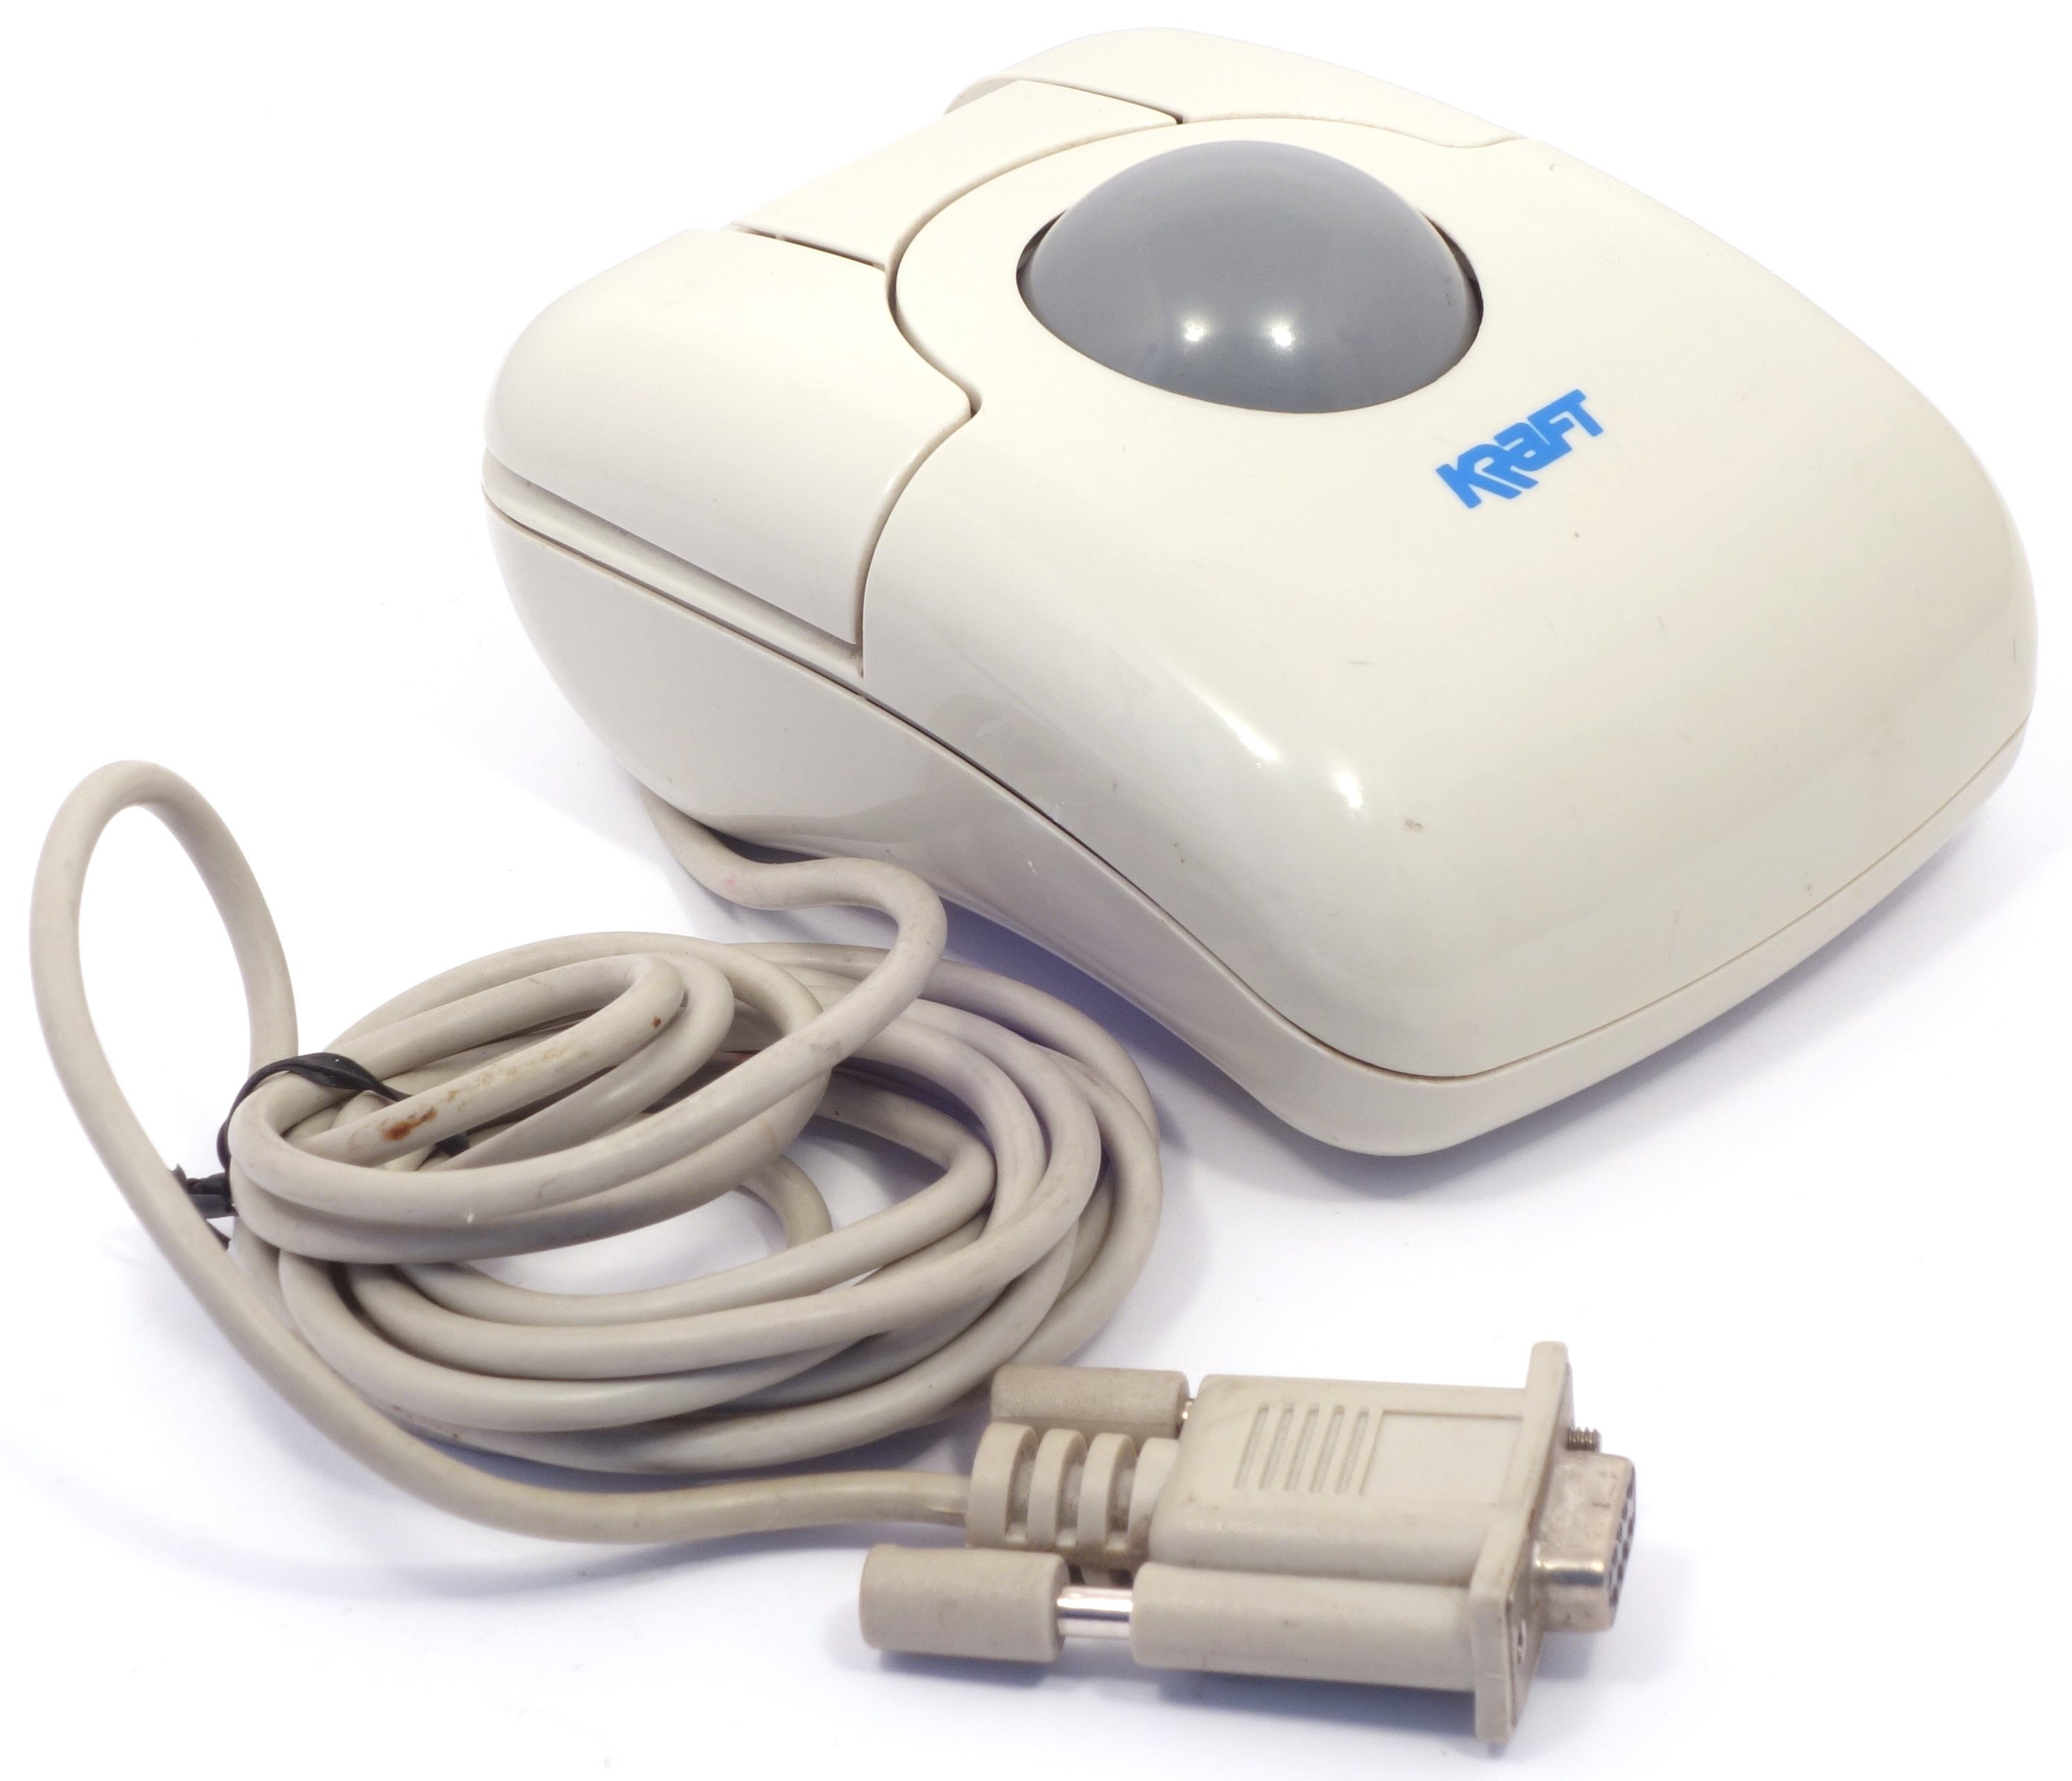
\includegraphics[scale=0.45]{1990_kraft_toptrack/pic_60.jpg}
    \caption{Kraft TopTrak trackball}
    \label{fig:TopTrakPic}
\end{figure}

The device is equipped with a 2.5 m cable, which is much longer than the typical distance between the user and the system unit. The trackball has a serial connection interface.

\begin{figure}[h]
    \centering
    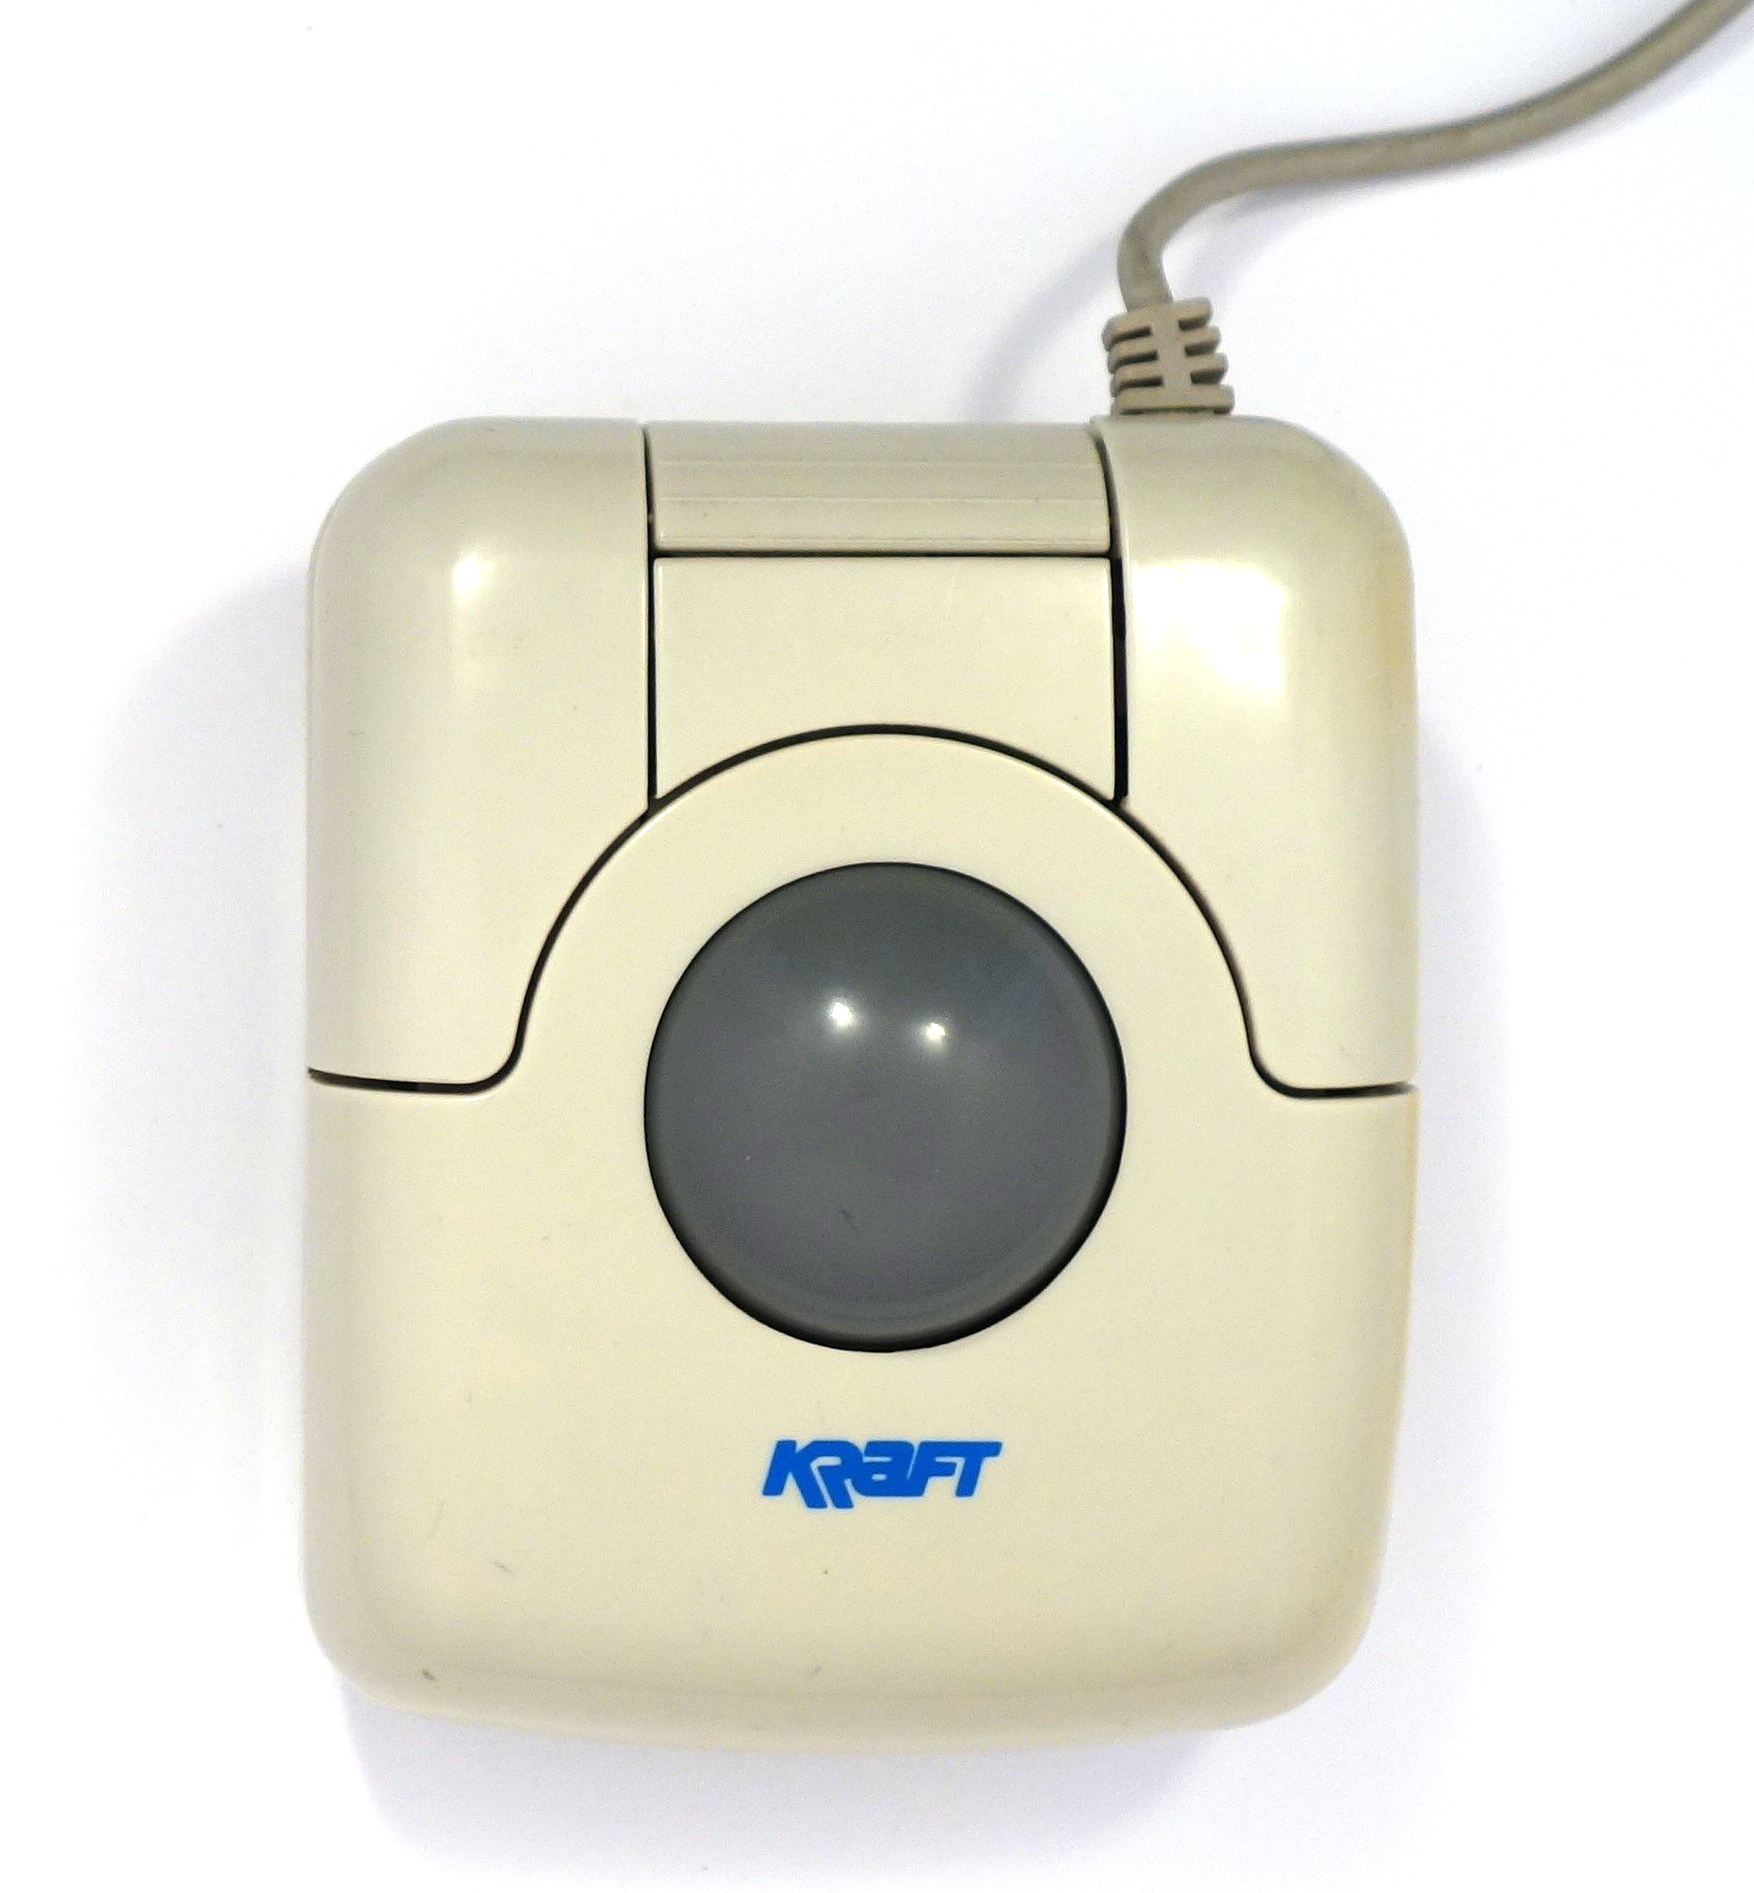
\includegraphics[scale=0.4]{1990_kraft_toptrack/2.9_60.jpg}
    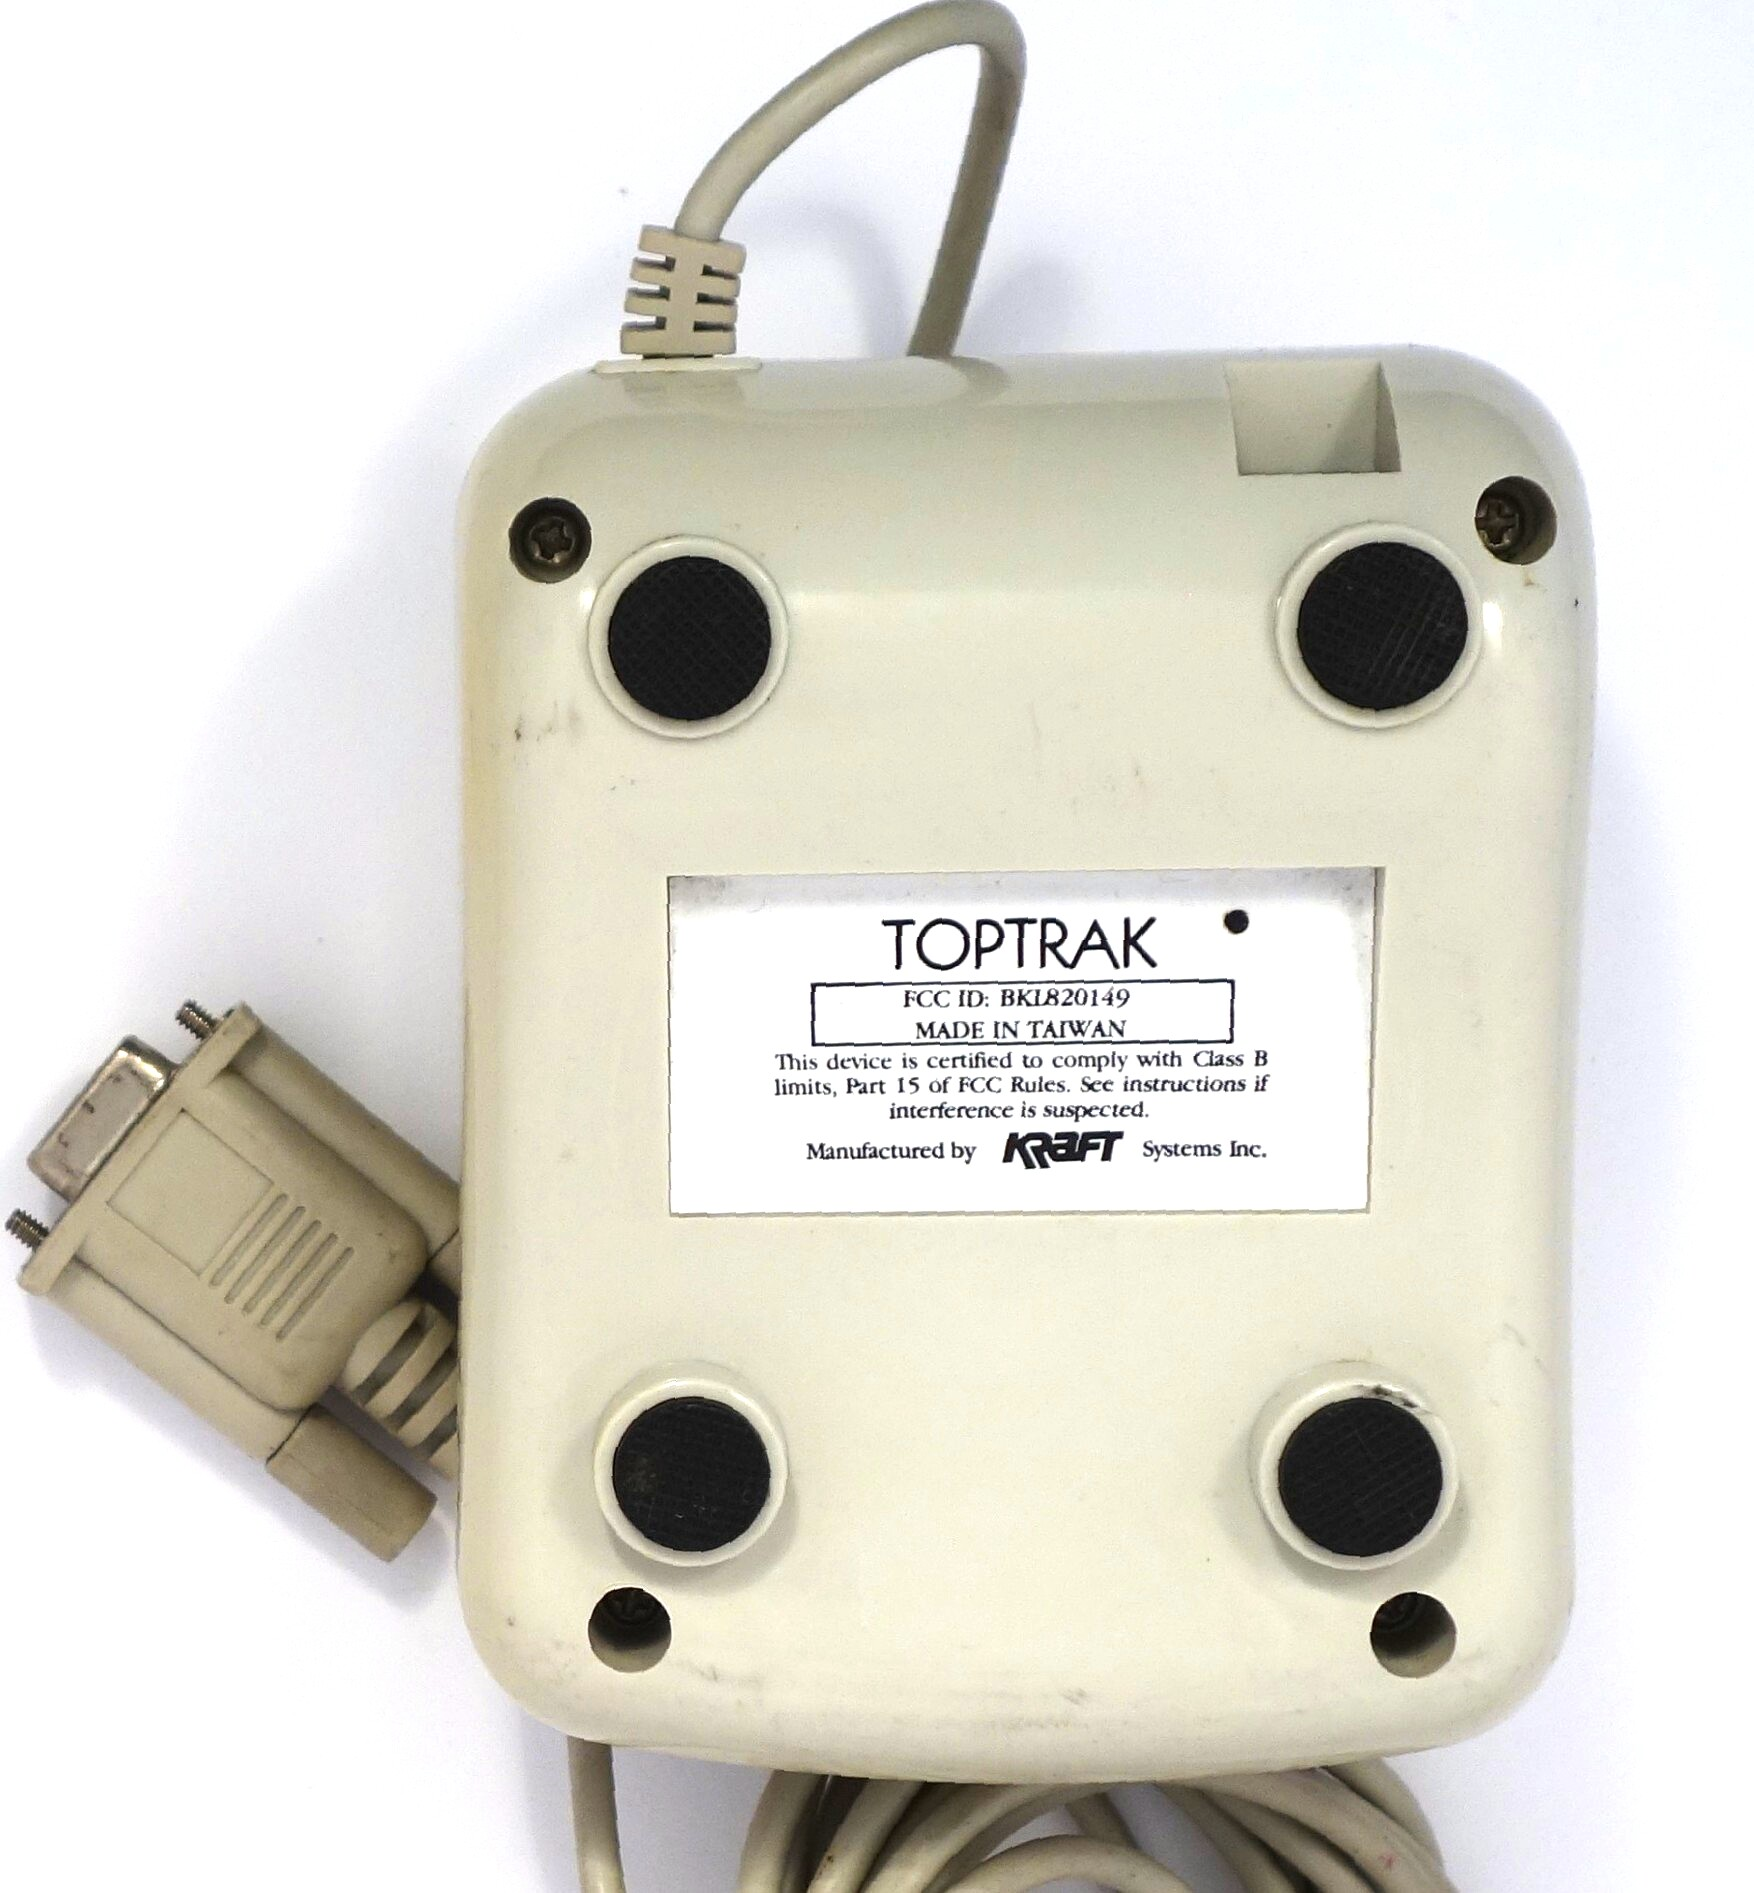
\includegraphics[scale=0.4]{1990_kraft_toptrack/2.10_60.jpg}
    \caption{TopTrak, top and bottom views}
    \label{fig:TopTrakTopAndBottom}
\end{figure}

Additionally, the trackball comes with a steel foot pedal (figure \ref{fig:TopTrakPedal}), which duplicates the left mouse button and adds another long cable and half a kilo of weight \cite{mouses} to the device.

\begin{figure}[h]
    \centering
    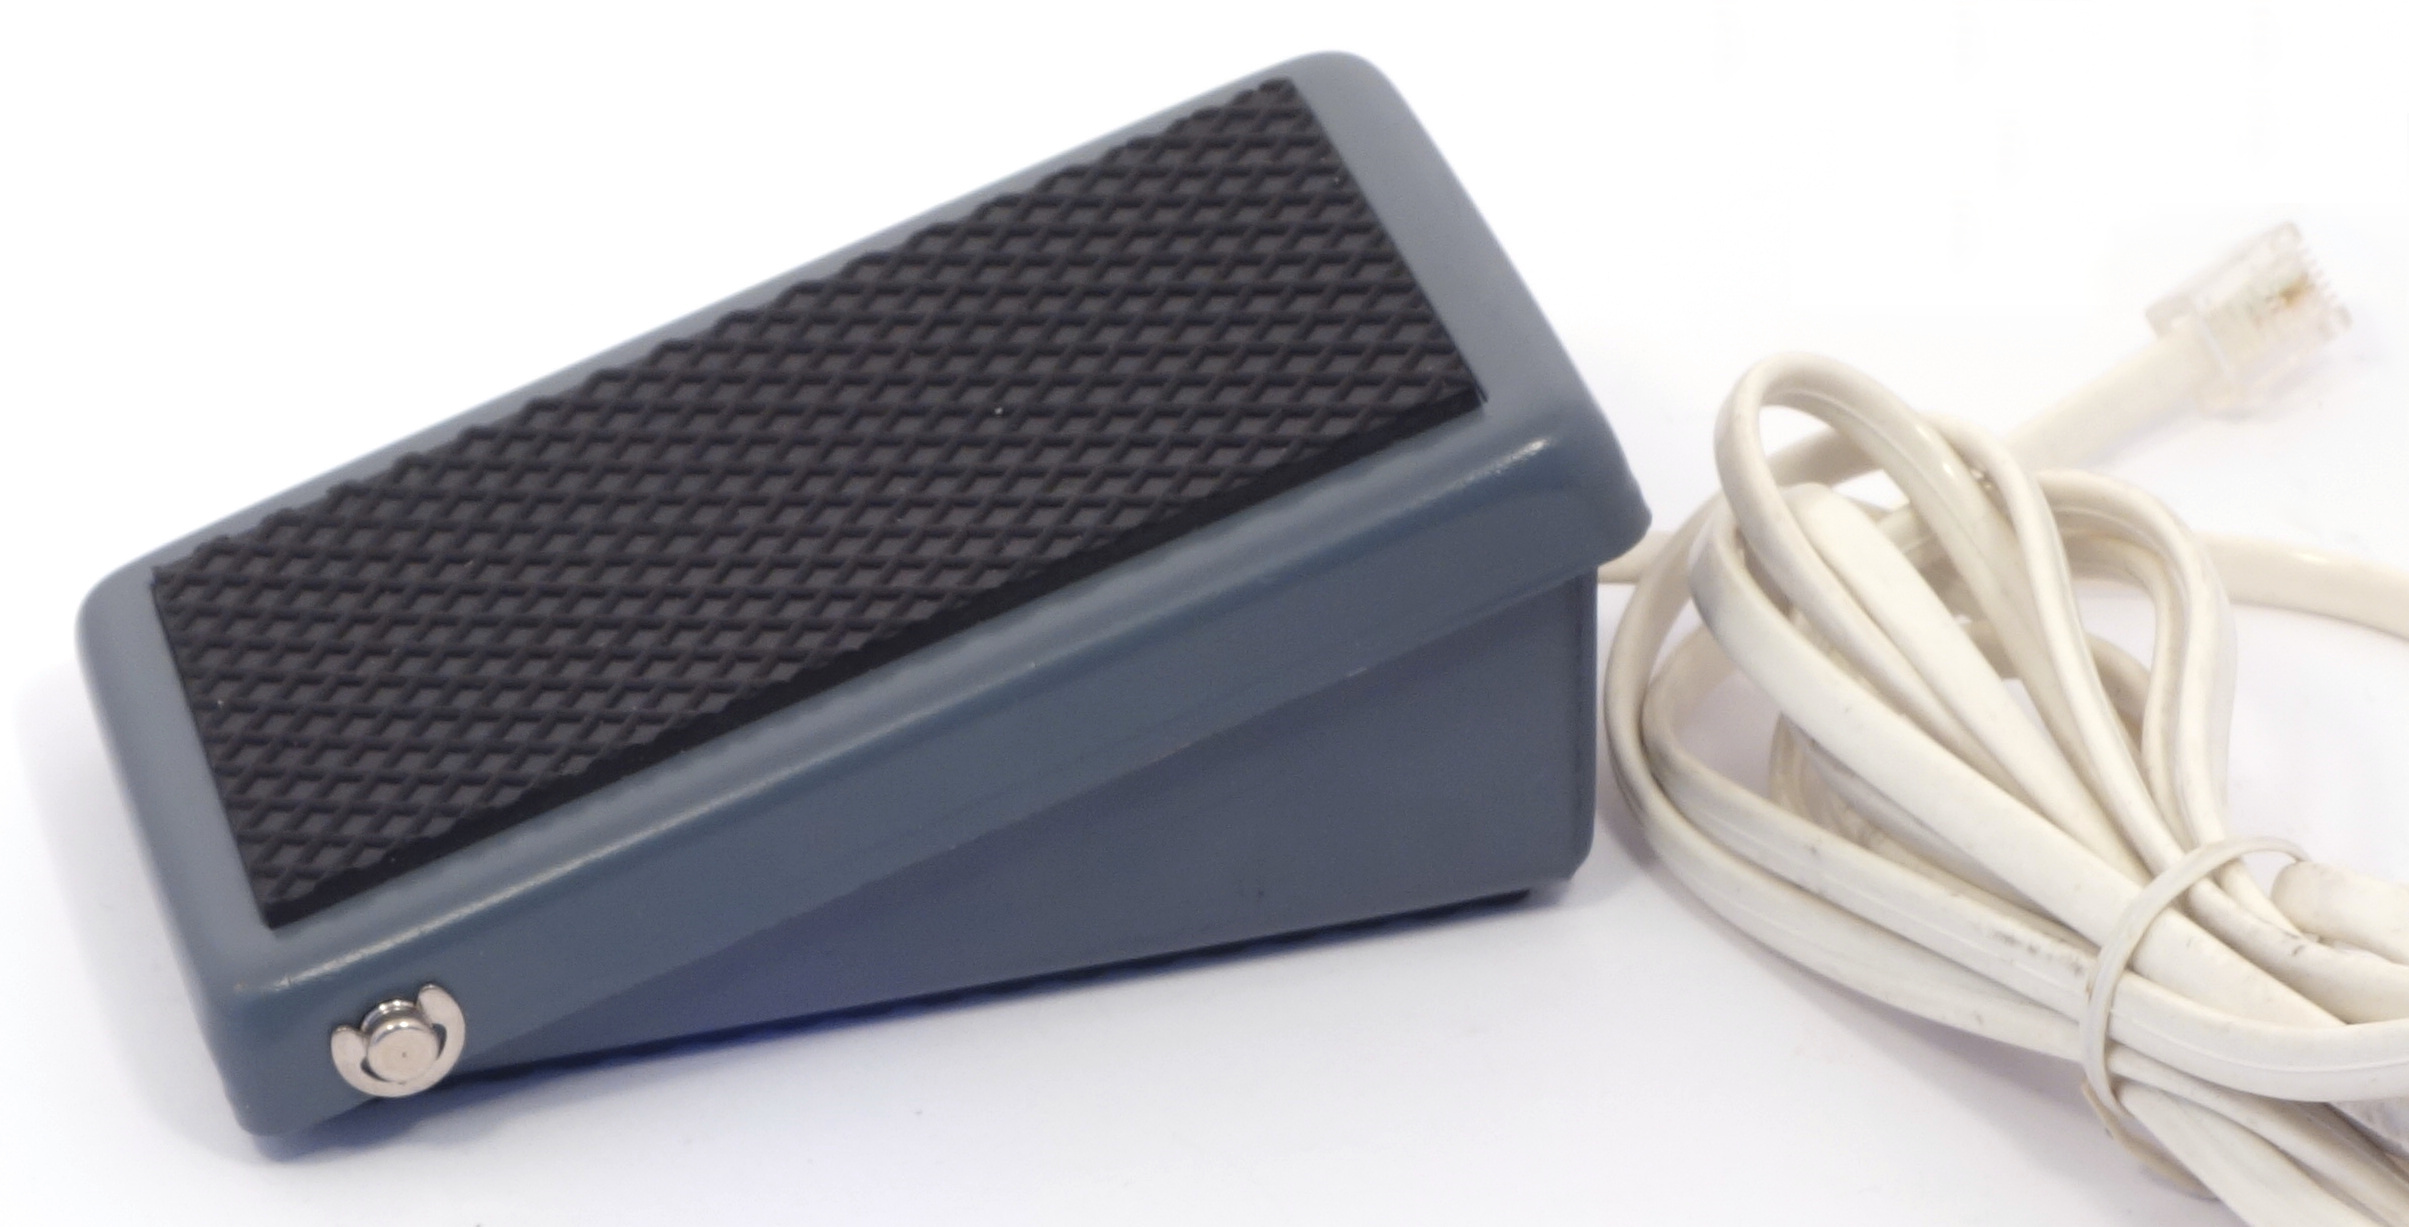
\includegraphics[scale=0.45]{1990_kraft_toptrack/pedal_30.jpg}
    \caption{Kraft TopTrak pedal}
    \label{fig:TopTrakPedal}
\end{figure}

%\begin{figure}[h]
%    \centering
%    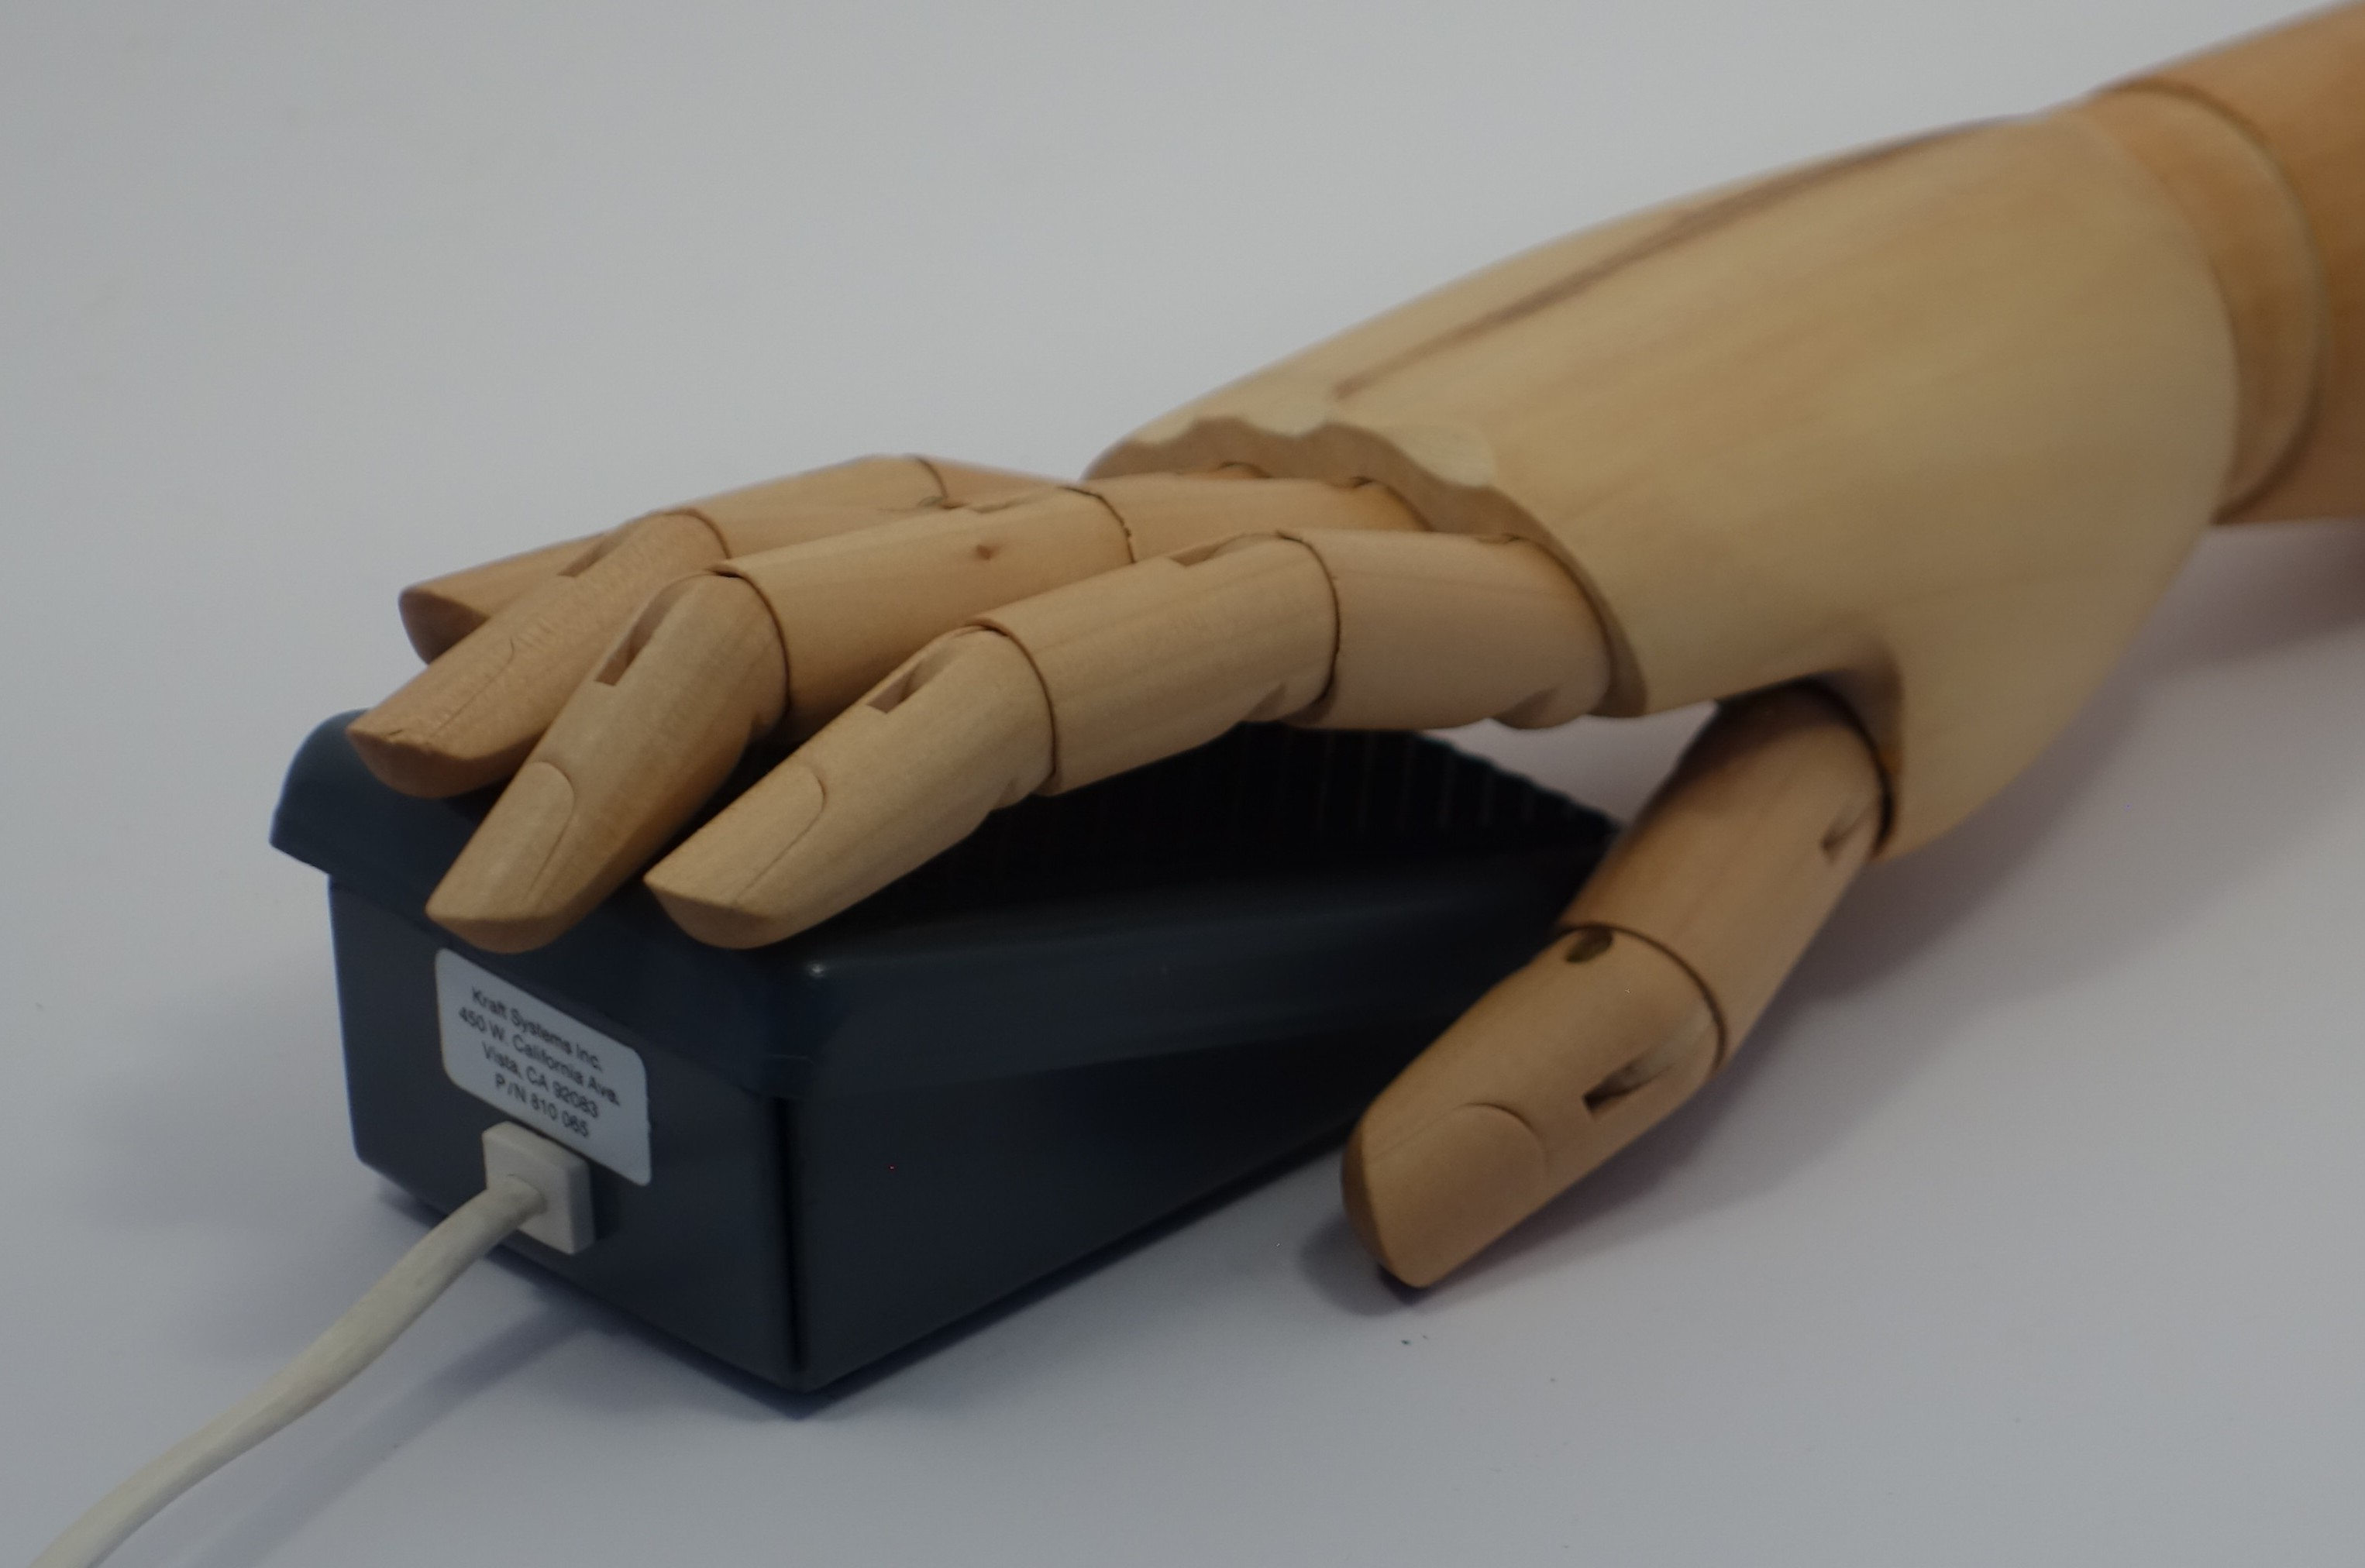
\includegraphics[scale=0.4]{1990_kraft_toptrack/2.8.jpg}
%    \caption{Kraft TopTrak pedal with a human hand model}
%    \label{fig:TopTrakPedalHand}
%\end{figure}

The Kraft TopTrak is a fairly compact device (figure \ref{fig:TopTrakSize}), especially when compared to the previous Kraft trackball model released in 1989, which was significantly larger in size, had an accentuated angular body, and was equipped with exactly the same pedal.

\begin{figure}[h]
    \centering
    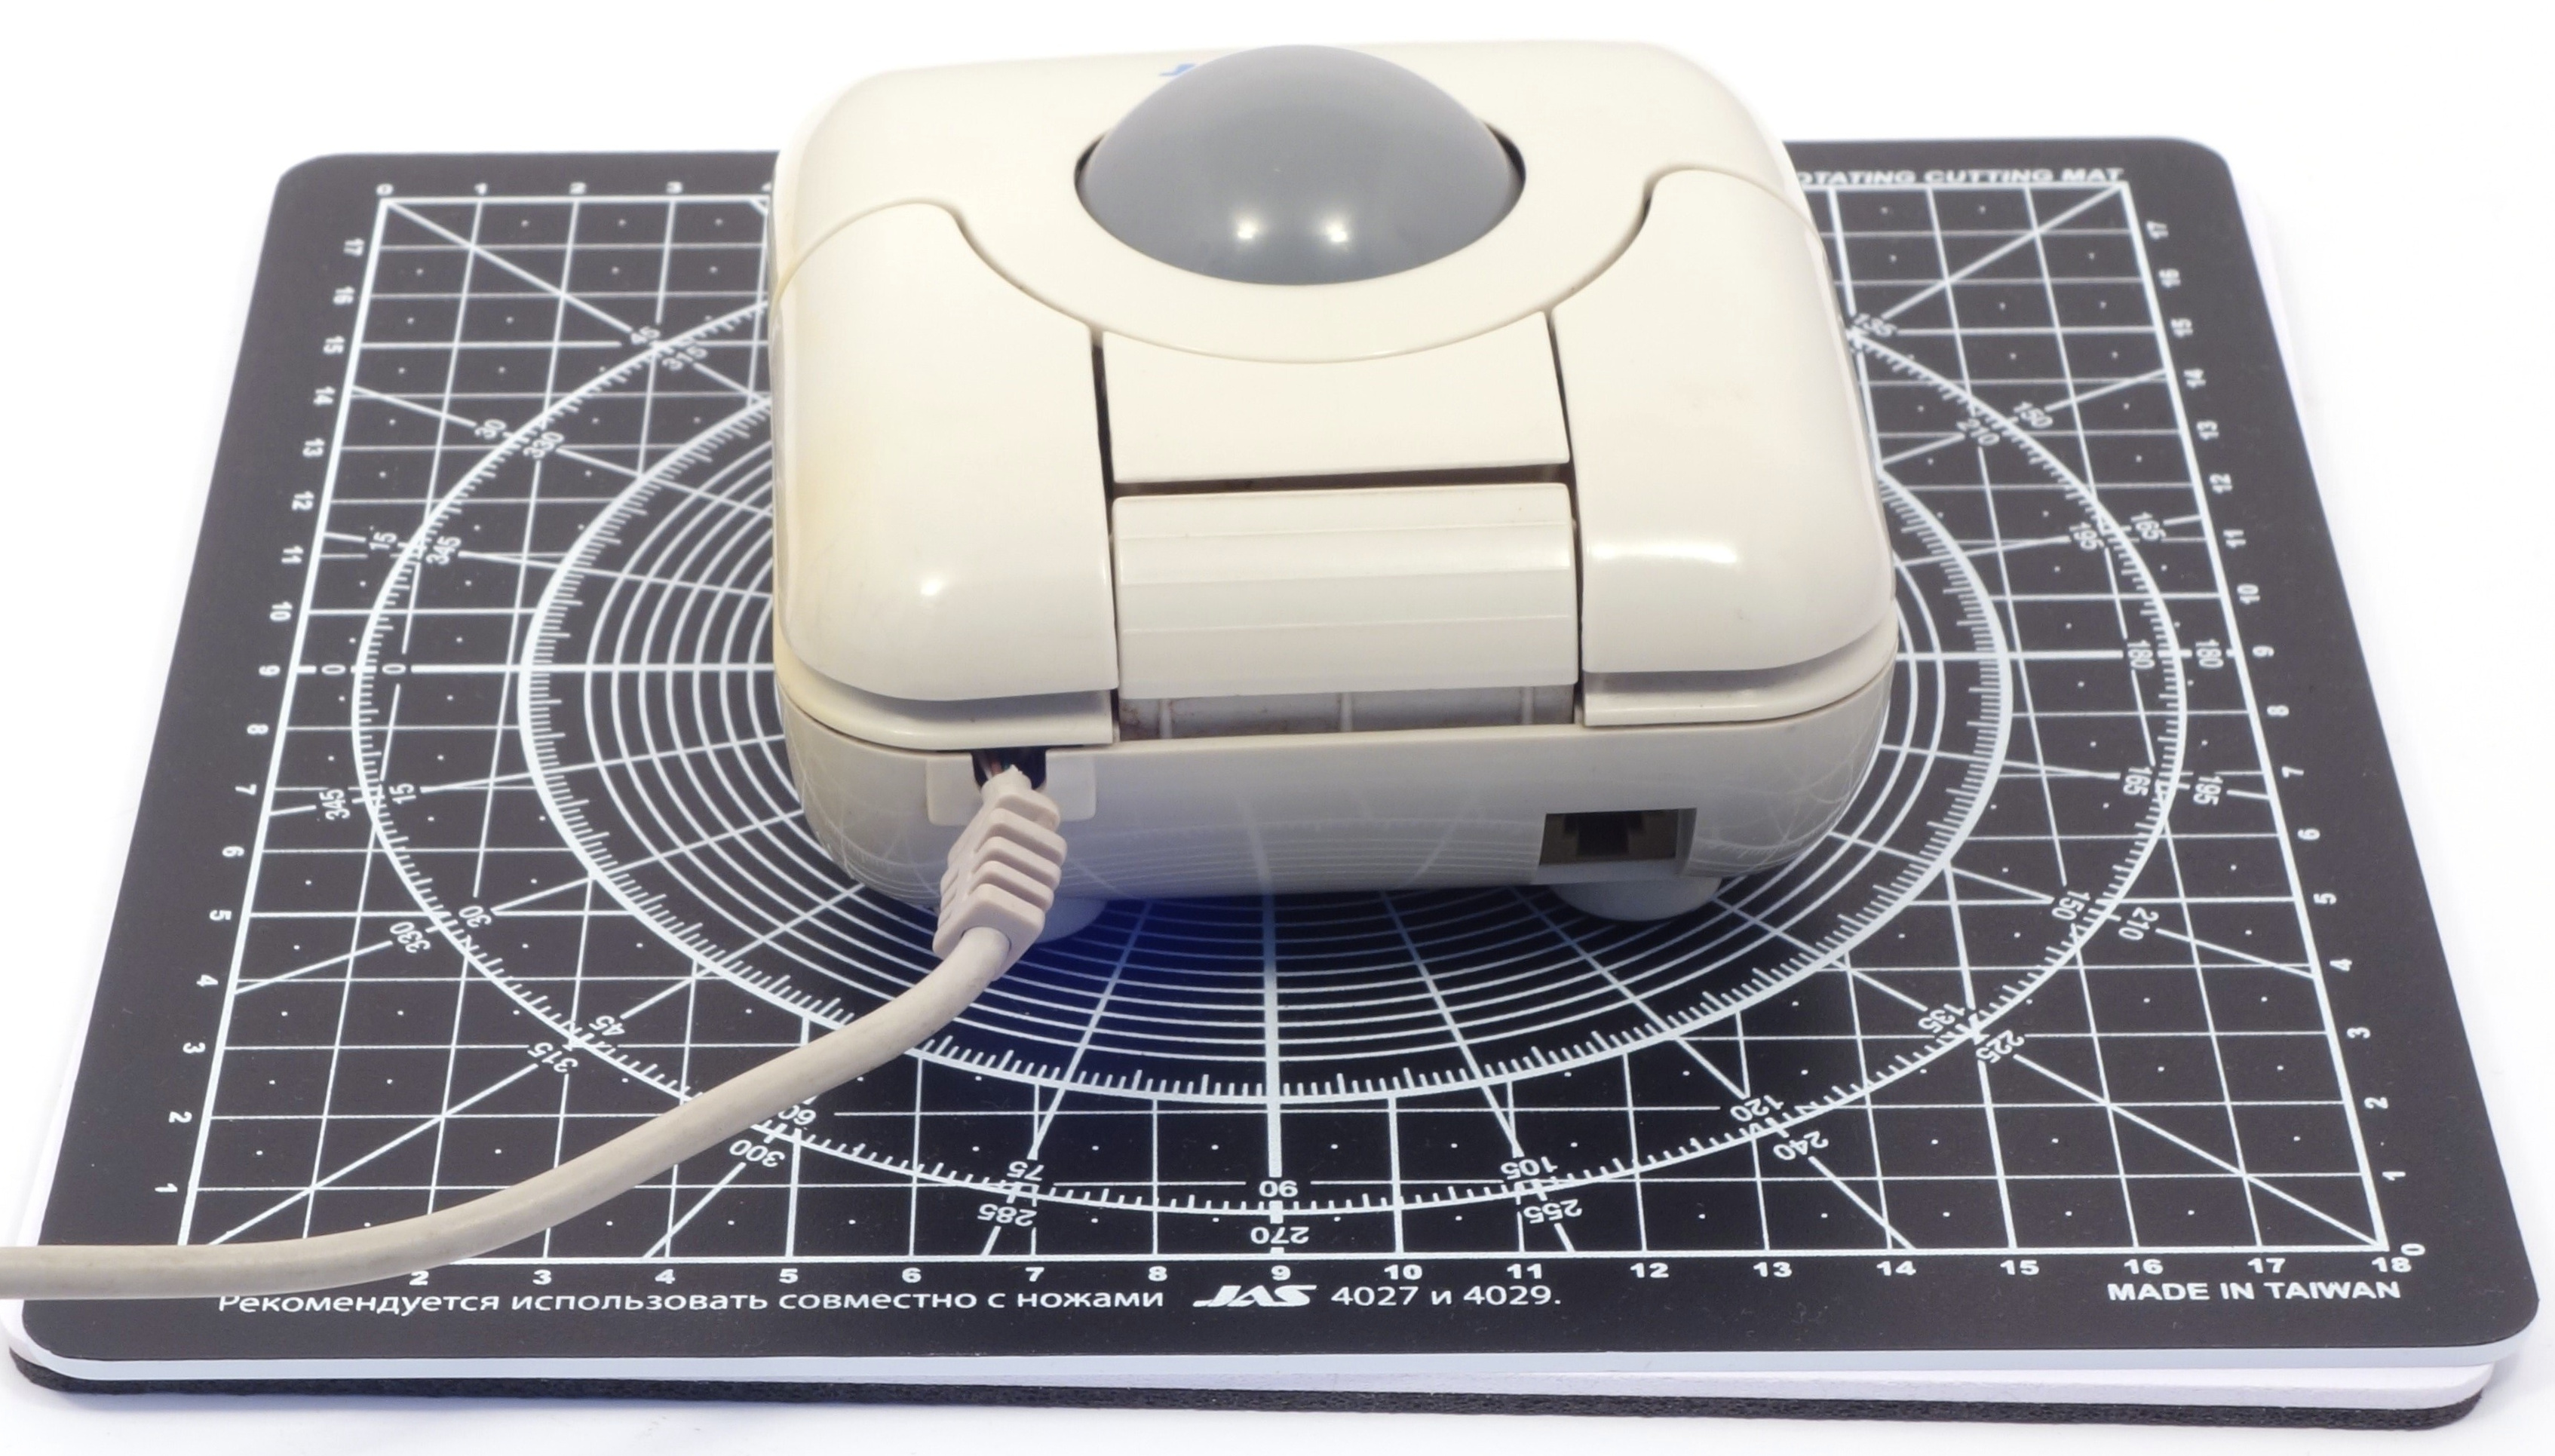
\includegraphics[scale=0.35]{1990_kraft_toptrack/2.6_30.jpg}
    \caption{TopTrak on a graduated pad with a grid step of 1~cm}
    \label{fig:TopTrakSize}
\end{figure}


The FCC ID code present on the TopTrak body (figure \ref{fig:TopTrakTopAndBottom}) shows that trackball was developed by the Kraft Systems company in 1990, just one year after the previous model.

In terms of ergonomics, the TopTrak is a significant step forward. The streamlined shape of the case, as well as large left and right buttons that completely occupy the upper corners, provide a fairly comfortable palm position (figure \ref{fig:TopTrakHand}).


\begin{figure}[h]
    \centering
    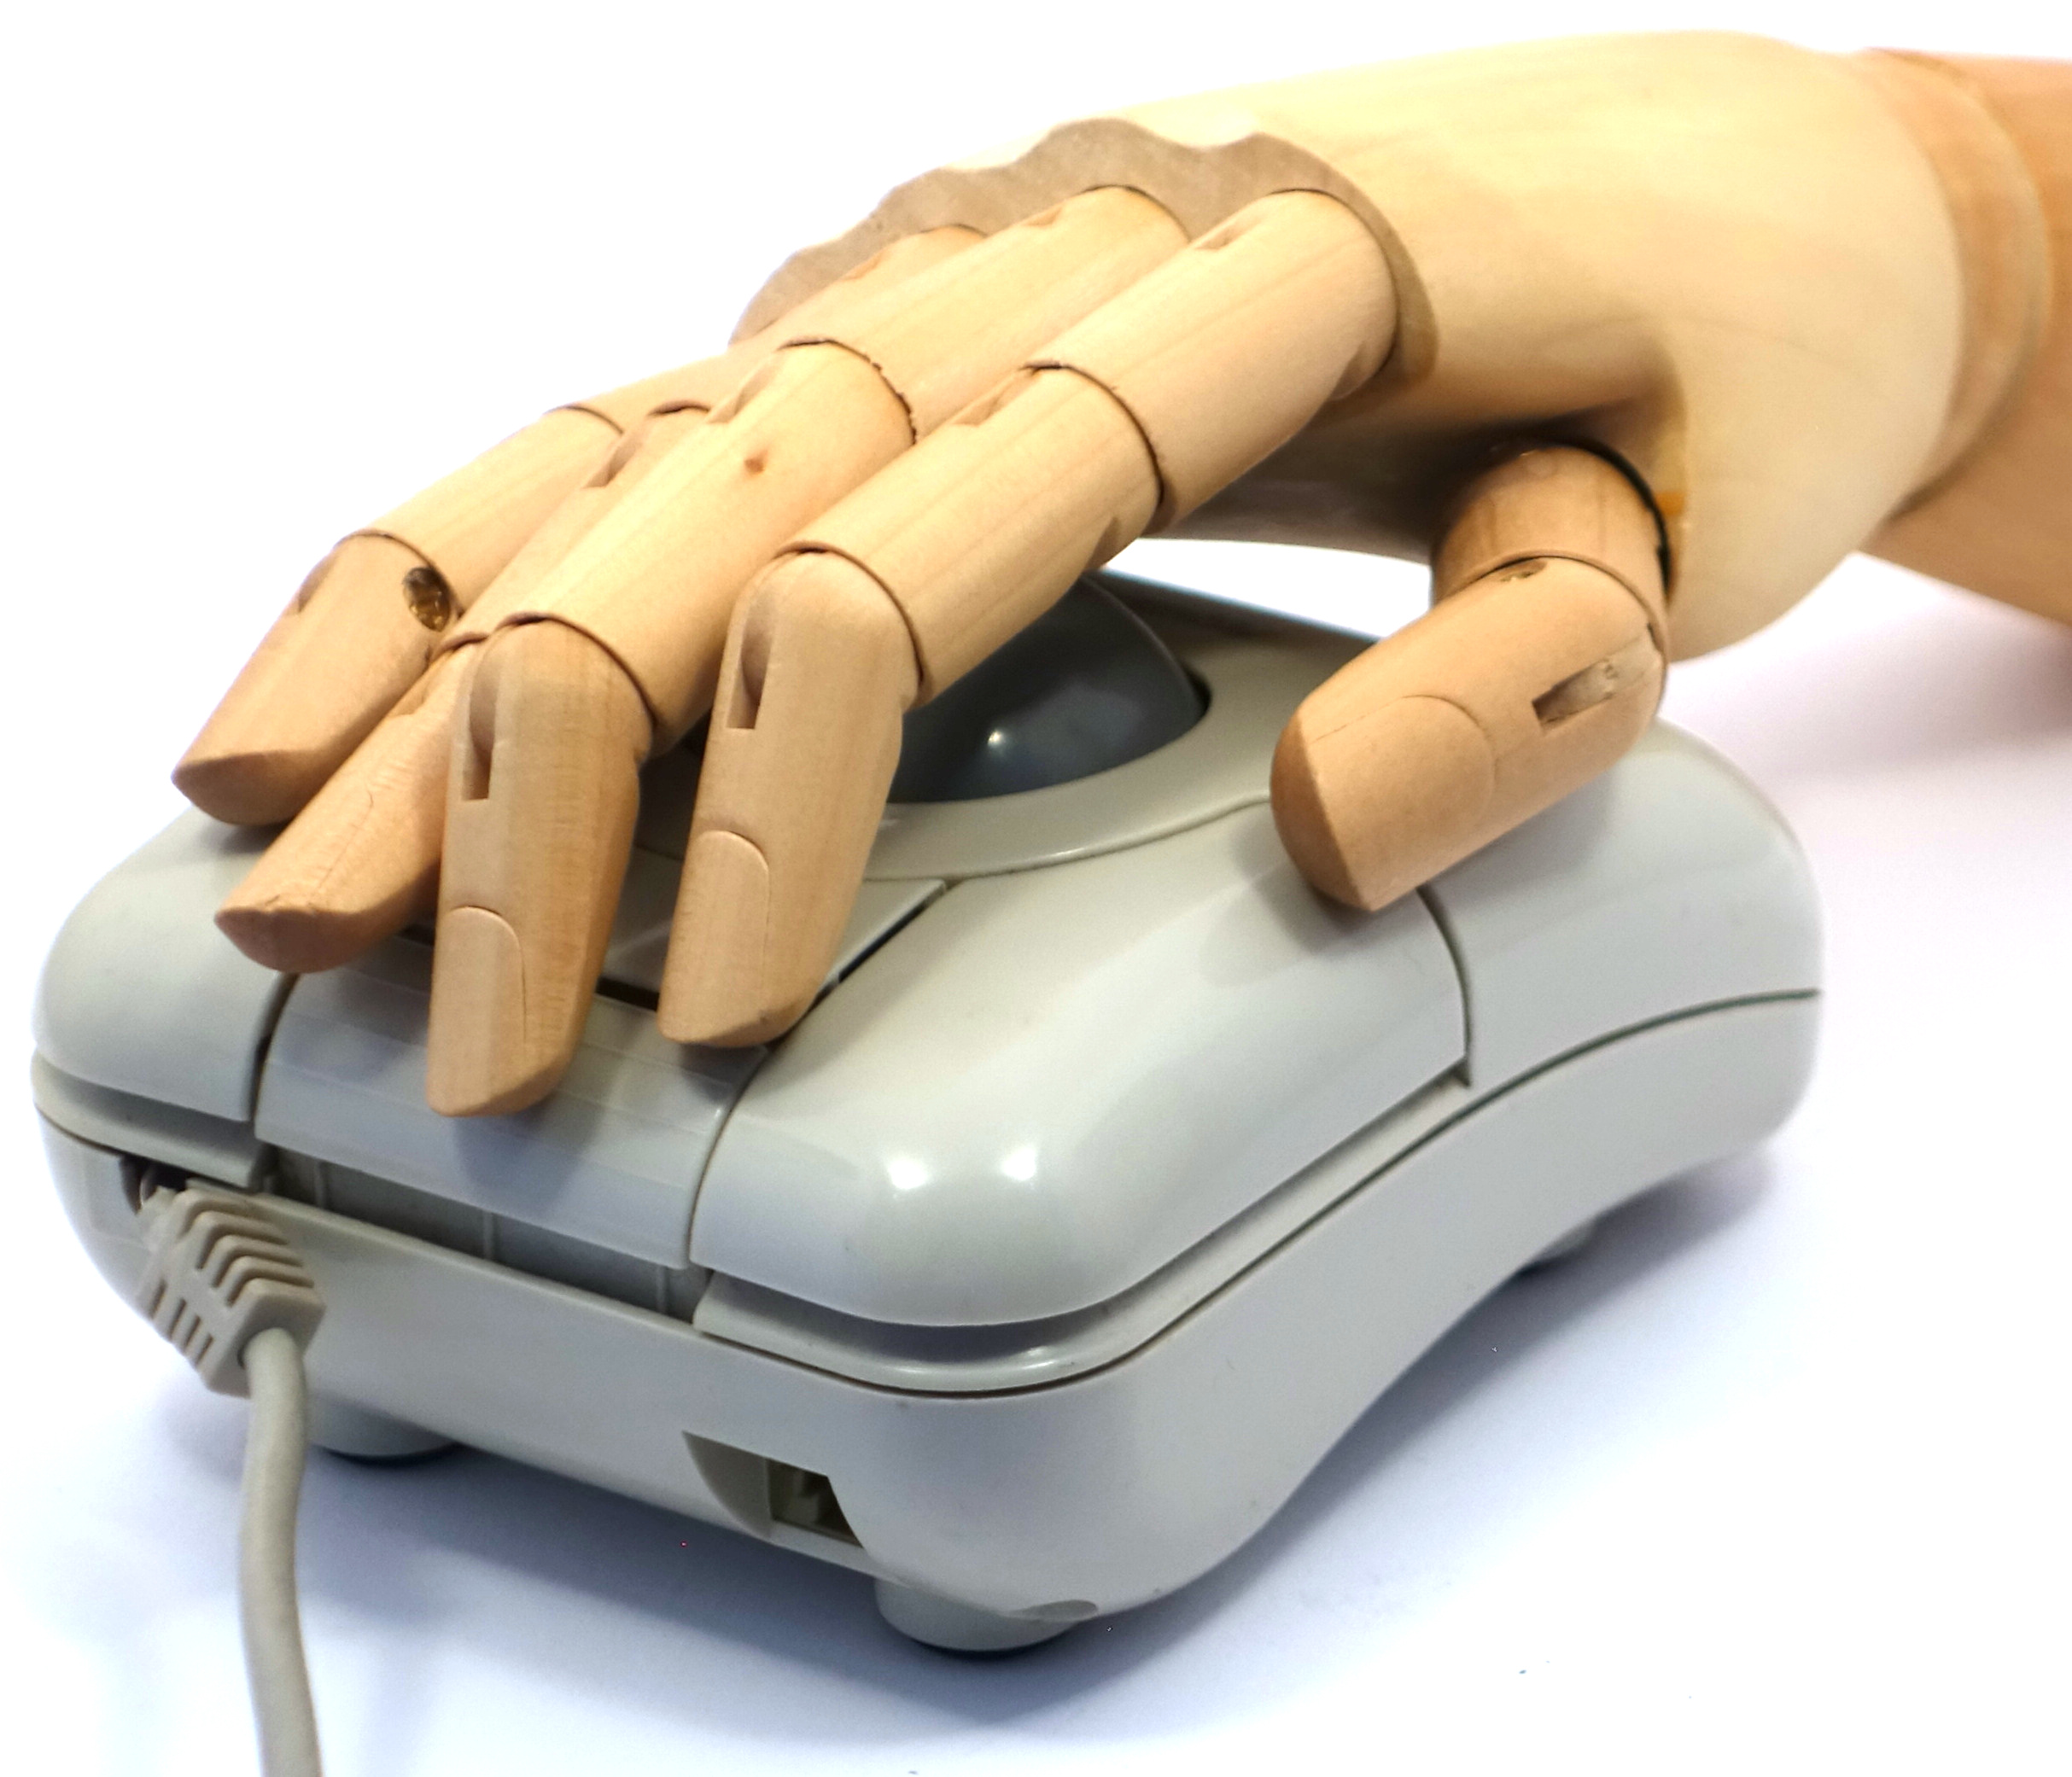
\includegraphics[scale=0.45]{1990_kraft_toptrack/hand_60.jpg}
    \caption{TopTrak with a human hand model}
    \label{fig:TopTrakHand}
\end{figure}


%\begin{figure}[htpb]
%    \centering
%    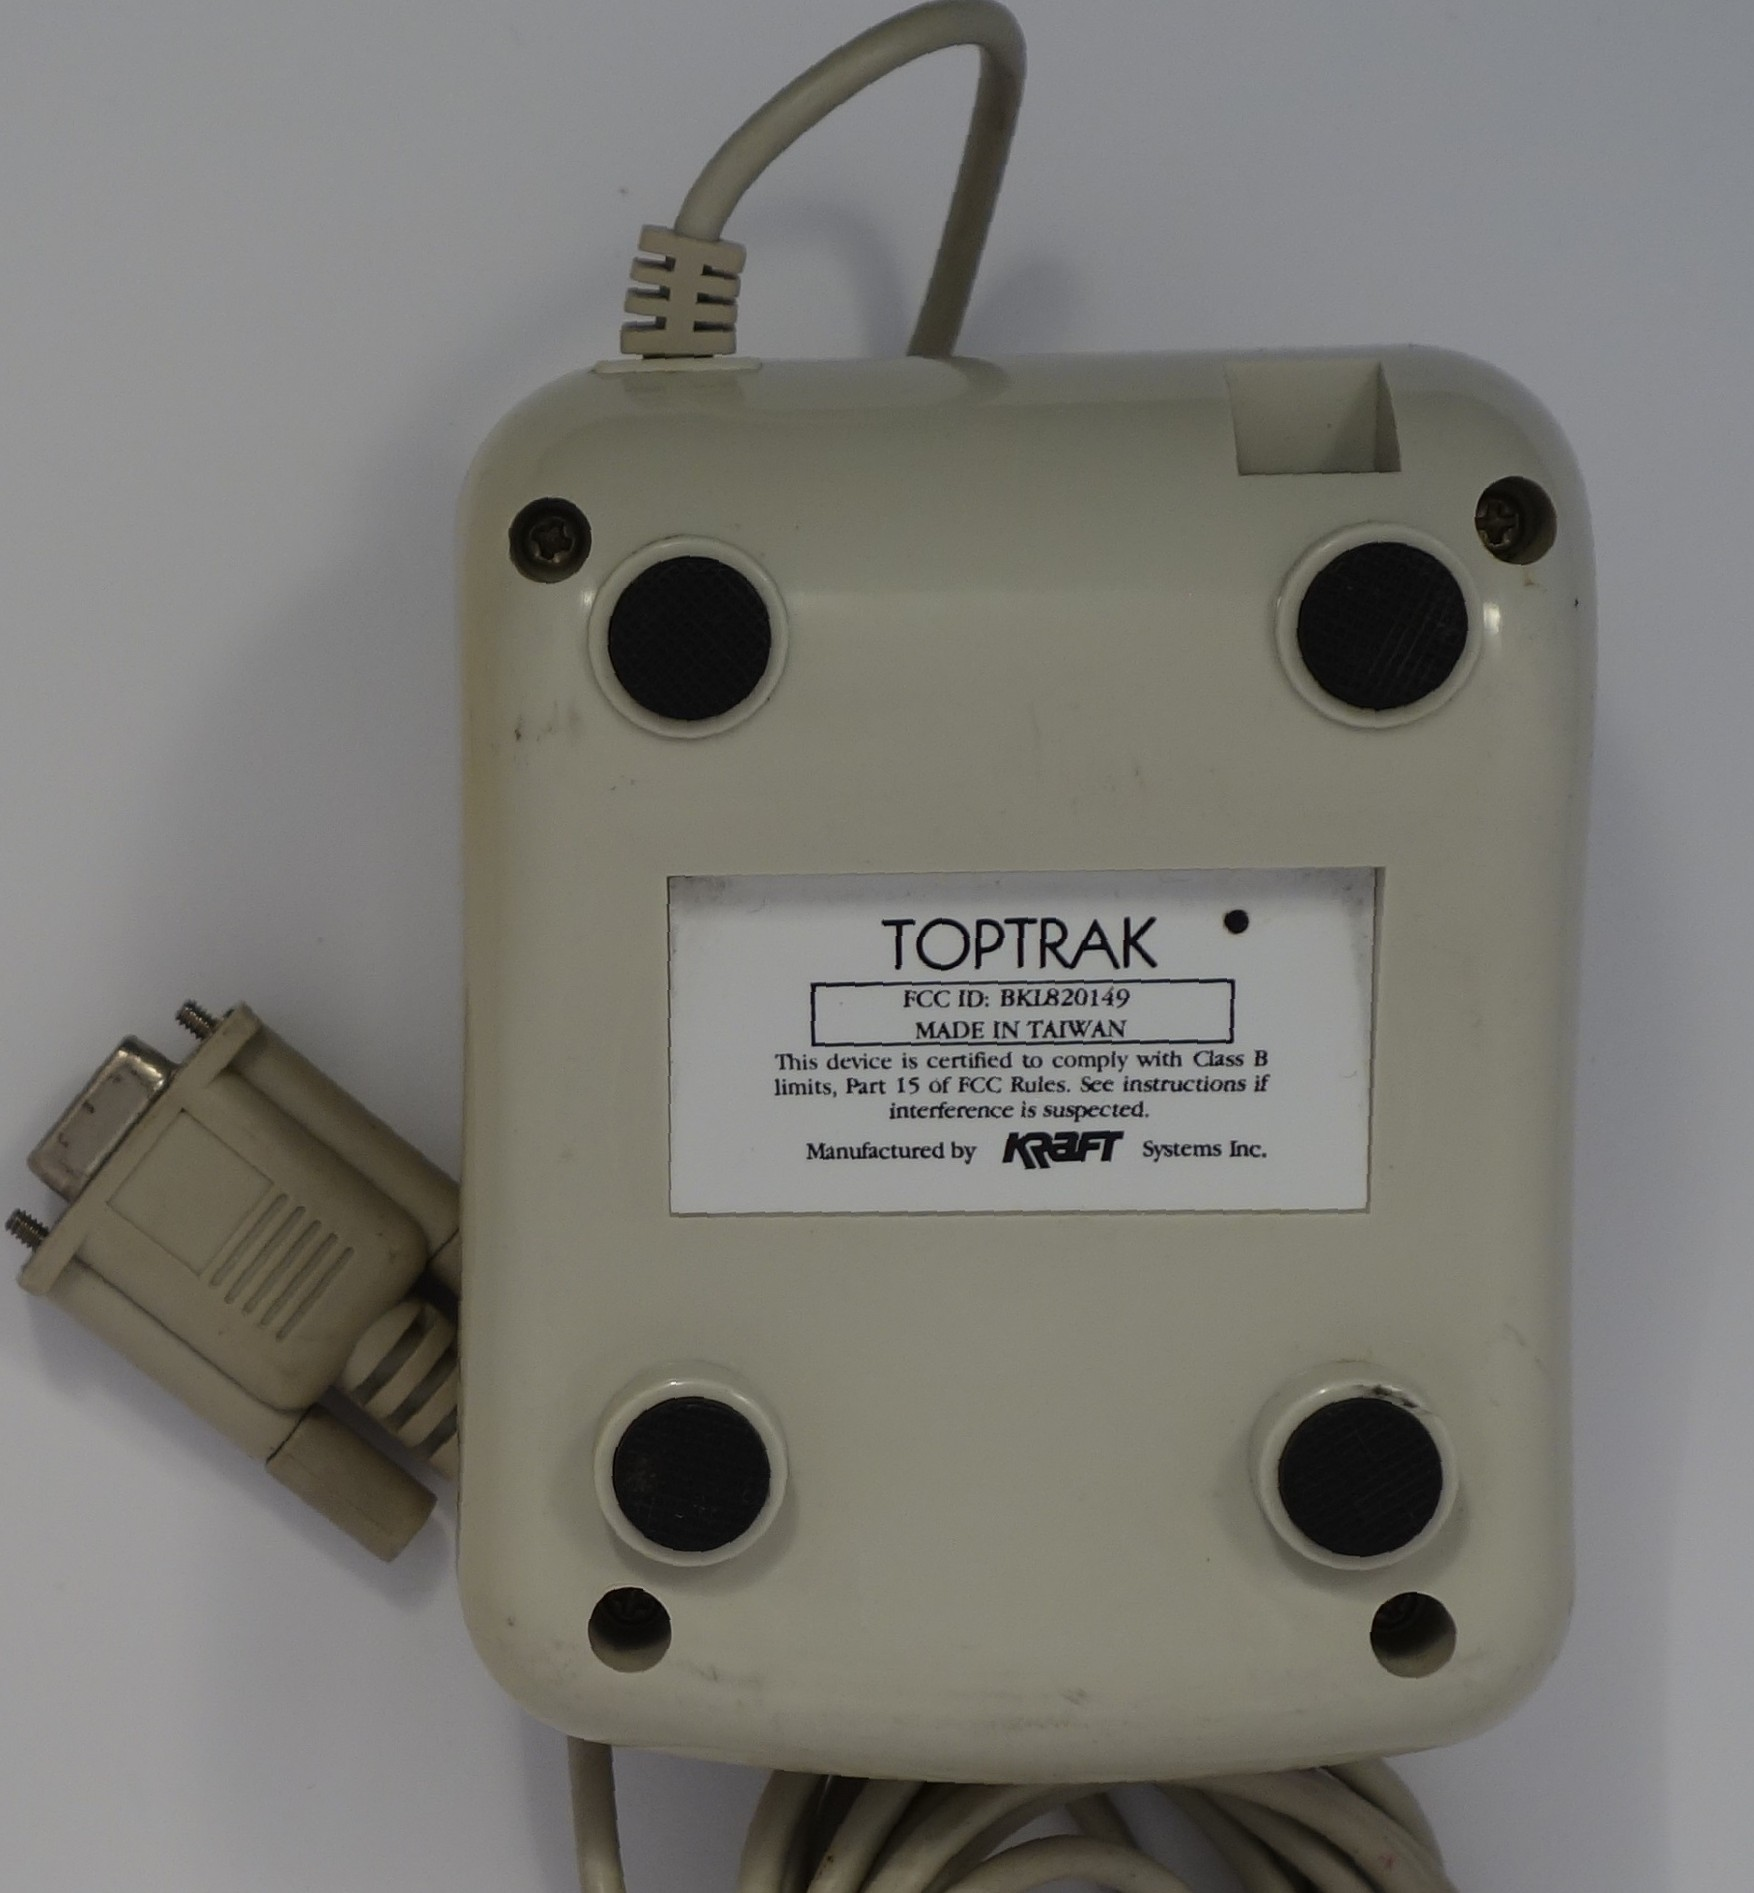
\includegraphics[scale=0.4]{1990_kraft_toptrack/2.10.jpg}
%    \caption{TopTrak, вид снизу}
%    \label{fig:TopTrakBottom}
%\end{figure}

Trackball internals are shown on figure \ref{fig:TopTrakInside}. The standard opto-mechanical design is supplemented by massive metal rollers with rolling bearings makes it clear that it was designed as a rather durable device, not for the low price segment.

\begin{figure}[h]
    \centering
    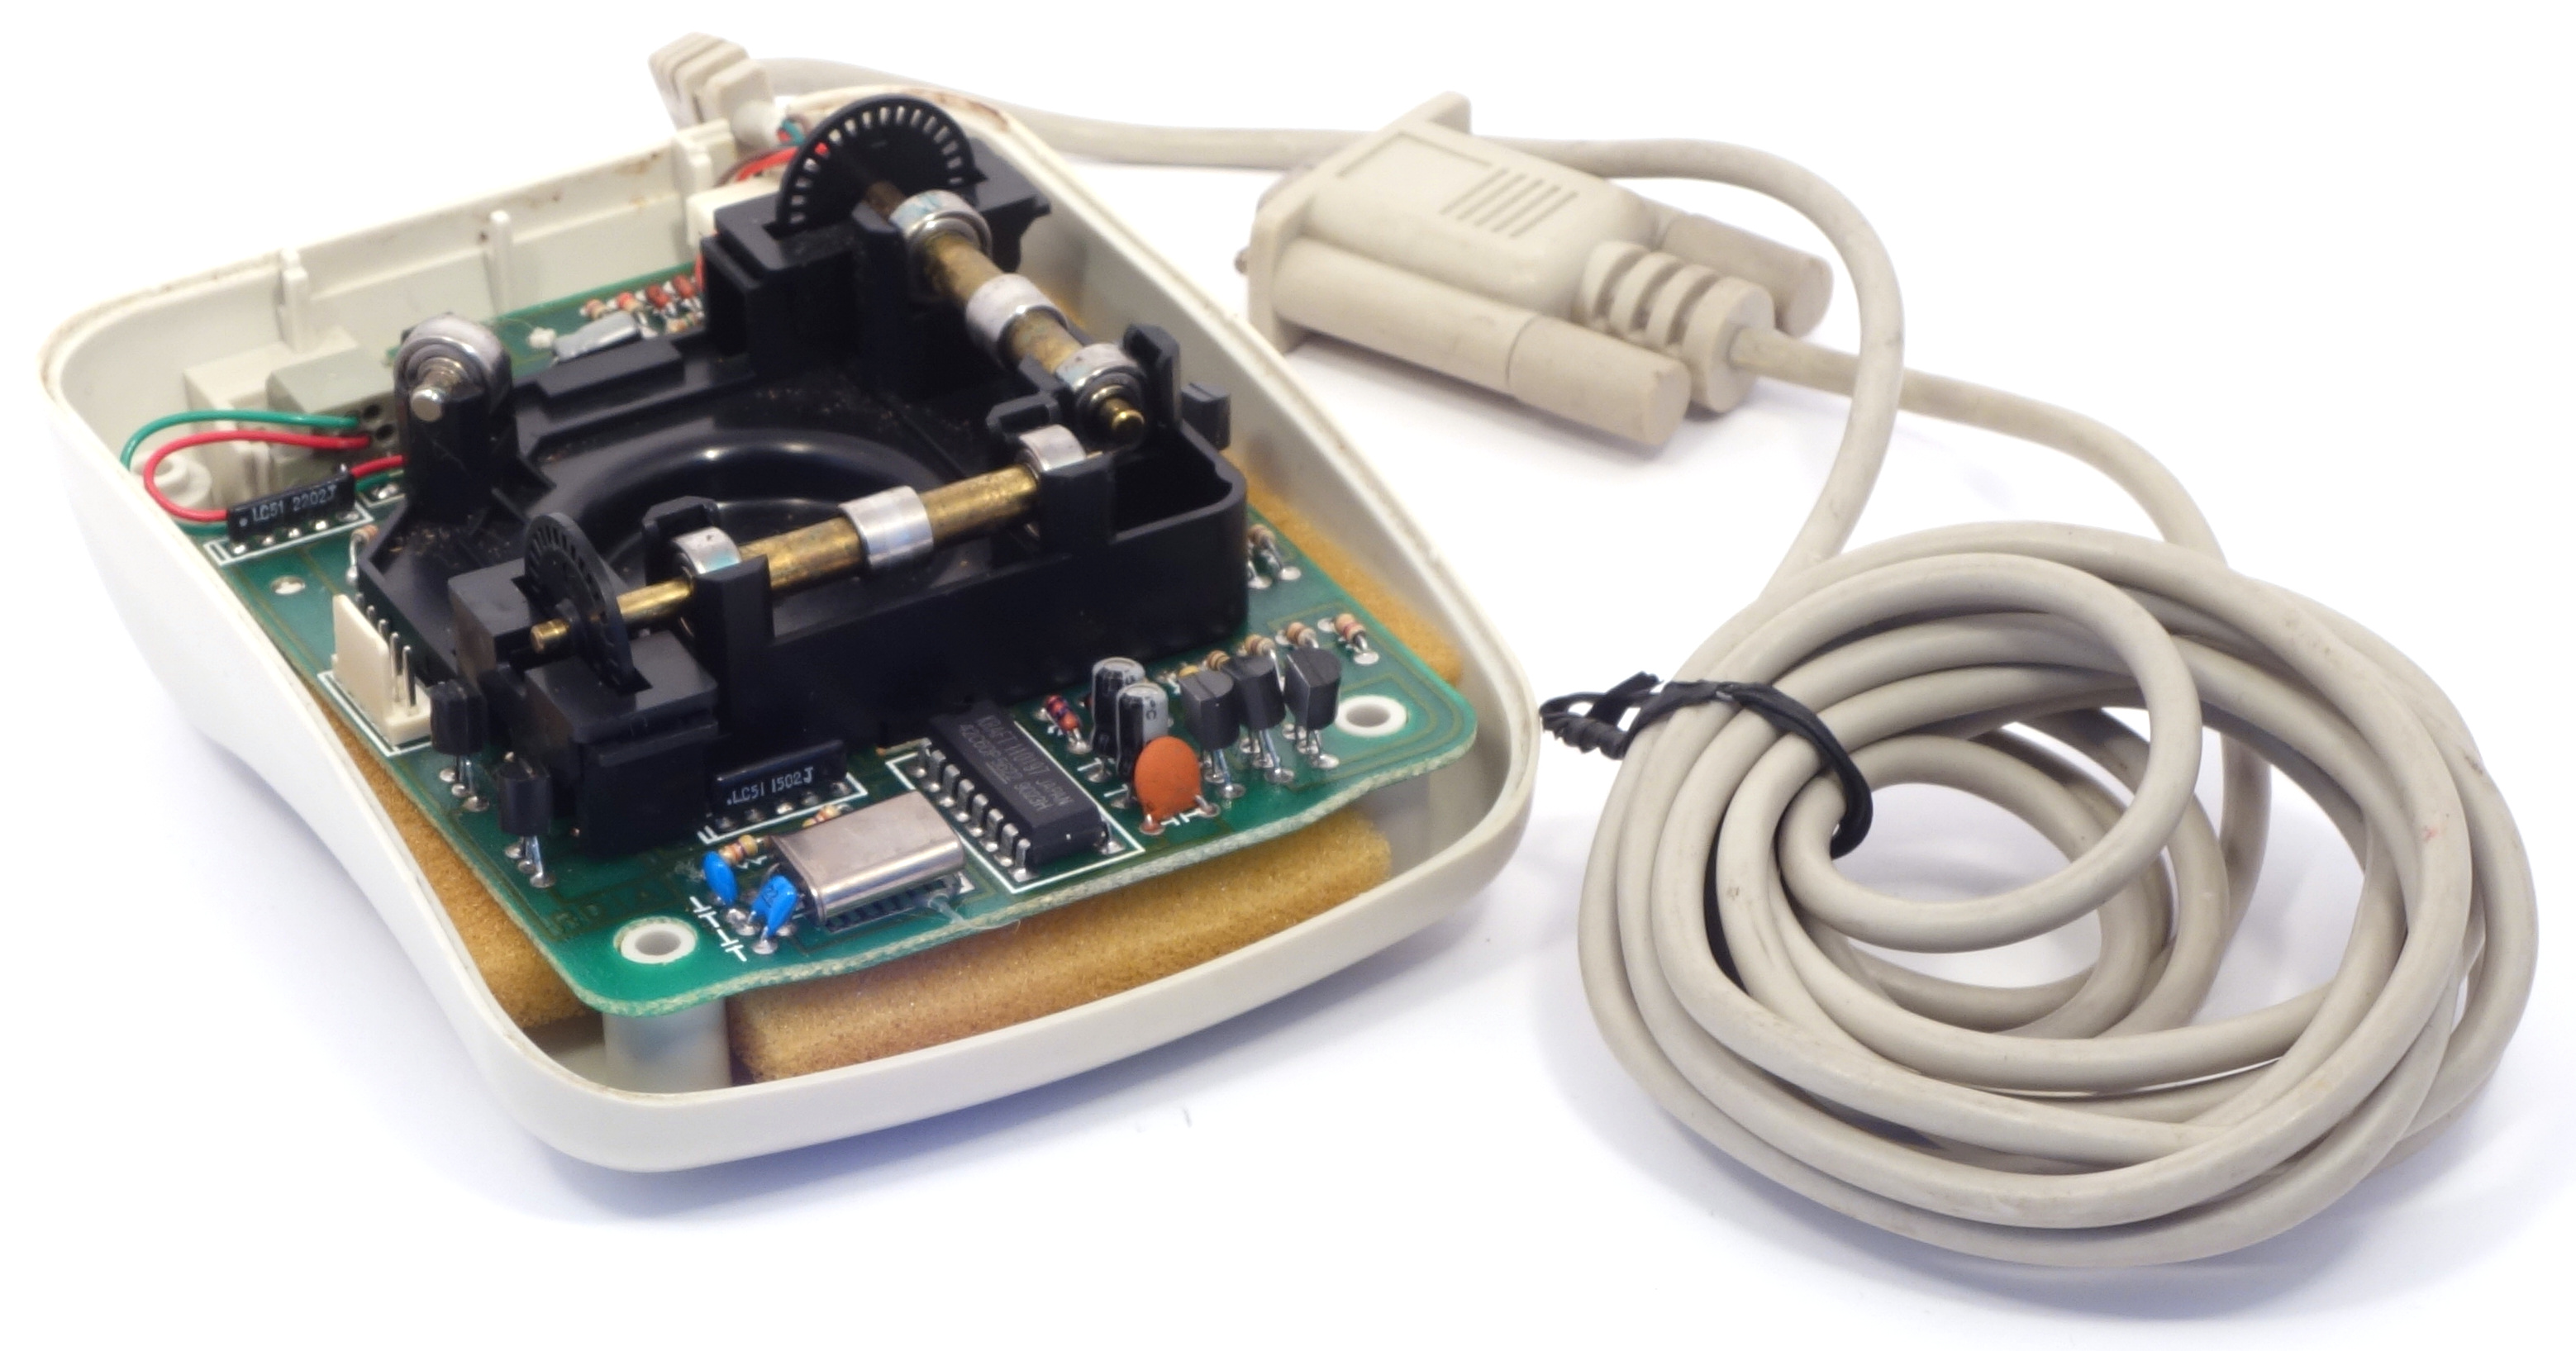
\includegraphics[scale=0.7]{1990_kraft_toptrack/inside_60.jpg}
    \caption{TopTrak disassembled}
    \label{fig:TopTrakInside}
\end{figure}

\begin{thebibliography}{9}
\bibitem {mouses} Berlin E. TopTrak // PC Magazine. October 15, 1991. p. 126-127 \url{https://books.google.by/books?id=tSLe3yMjc-AC&lpg=PP1&pg=PT123#v=onepage&q&f=false}
\end{thebibliography}
\end{document}
